\chapter{Opis projektnog zadatka}
		
		%\textbf{\textit{dio 1. revizije}}\\
		
		Cilj projekta „Djeca za djecu“ je razviti web aplikaciju koja će omogućiti roditeljima, i onim budućim, da lakše doniraju i pronalaze donacije za svoju djecu. \\
		\newline
		U doba kada su već i osnovne namirnice preskupe i globalno zagađenje raste, „recikliranje“ predmeta postaje još važnije. Zašto bacati dobro očuvane stvari koje još mogu poslužiti nekome i spasiti njegov džep, a nemamo ih gdje čuvati dok ne zatrebaju kolegi/prijateljima/rodbini…  \\
		\newline
		Ova aplikacija brzo i efikasno spaja donatora i primatelja donacije bez da korisnici moraju pretraživati bespuća interneta. Oglasi u aplikaciji prilagođavaju se profilu korisnika. Nakon što korisnik jednom upiše svoje podatke i podatke o svojoj djeci, automatski mu se prikazuju oglasi od interesa. Dodatno se mogu namještati filteri kategorija kod pregleda oglasa. \\
		\newline
		Doniranje, također, nikada nije bilo lakše. Nakon što korisnik objavi oglas za predmet, više se ne mora brinuti o njemu dok aplikacija sama ne pronađe savršenog primatelja. Tek kada predmet pronađe svog potencijalnog novog vlasnika zamišljeno je da primatelj kontaktira donatora izvan aplikacije te se dogovori za primopredaju. Nakon izvršene donacije donator treba samo potvrditi da je donirao korisniku upisivanjem mail adrese primatelja.\\
		\newline
		Sigurnost i kredibilitet aplikacije i oglasa važni su za iskustvo korisnika. Stoga je aplikacija zatvorena na registrirane korisnike što omogućava praćenje aktivnosti unutar aplikacije. Provode se provjere na razini korisnika i oglasa. Korisnici (ADMIN van aplikacije) se provjeravaju na temelju prijašnjih donacija ili postojećih zapisa o njima kako bi eliminirali moguće prevare ostalih korisnika aplikacije. Oglasi, pak, moraju biti opisani u skladu sa standardom aplikacije i predmeti ne stariji od preporučene starosti za određen predmet.
		\newline

		\eject
		Istraživanjem hrvatskog „tržišta“ za sličnim aplikacijama pokazalo se da ne postoje aktivne aplikacije za doniranje i razmjenu dječjih stvari. U 2017. godini govorilo se o BIPO CLUB aplikaciji (poznatog BIPO branda za djecu, trgovačkog lanca BIPA) za razmjenu dječjih stvari koja trenutno više nije dostupna. Kako su odgovorili iz BIPO kluba, aplikacija se više ne koristi te su gašenjem iste spojili BIPO i BIPA kartice pa se više ne može aktivirati korisnički račun u aplikaciji.
		\begin{figure}[h!]
			\center
			
\includegraphics[width=\textwidth,height=0.2\textheight]{./slike/Picture1.png}
			\caption{Oglas za mobilnu aplikaciju BIPO CLUB}
			\label{fig1}
		\end{figure}
		\newline
		Za razliku od web aplikacije, vidimo da se ovdje radi o mobilnoj aplikaciji kompatibilnoj s IOS i Android uređajima, no slično našoj, postoje dvije funkcionalnosti dostupne korisniku - traženje i doniranje predmeta. \\
		\newline
		Registrirani korisnik može pregledavati oglase i primati donacije, ali i kreirati vlastite oglase i tim putem donirati dječje stvari koje mu više ne trebaju.\\
		
		\begin{figure}[h!]
			\center
			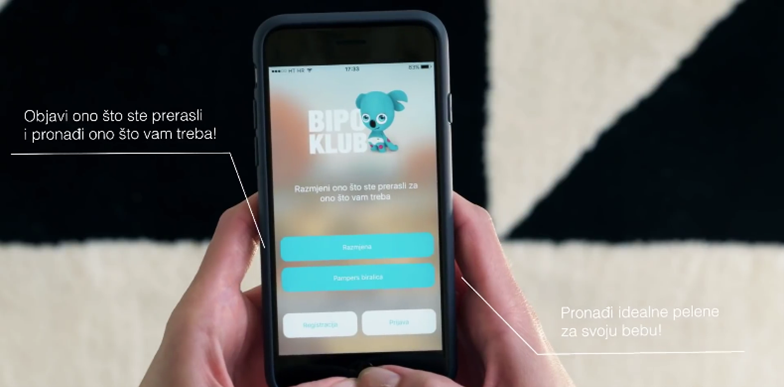
\includegraphics{./slike/Picture2.png}
			\caption{ "Landing page" aplikacije BIPO CLUB}
			\label{fig2}
		\end{figure}
		Slično aplikaciji koja će nastati u ovom projektu, aplikacija je zatvorena na registrirane korisnike, a na početnom zaslonu ima prijavu/registraciju korisnika. \\
		\newline
		U aplikaciji koju razvijamo neregistrirani korisnik će se jedino moći registrirati u sustav na početnom zaslonu, a registrirani prijaviti. Nakon registracije korisniku stiže mail potvrde te se ima pravo prijaviti sa svojim korisničkim računom. Ulaskom u aplikaciju korisnik dalje može birati hoće li uređivati/pregledavati svoj profil i/ili dodavati podatke o djeci koji se koriste za filtriranje preporučenog sadržaja. Primjerice, korisnik ima muško dijete u dobi od 3 godine - ako na svom profilu doda podatke o dobi i spolu svog djeteta, među preporučenim oglasima bit će samo predmeti za trogodišnjake.\\
		\newline
		\begin{figure}[h!]
			\center
			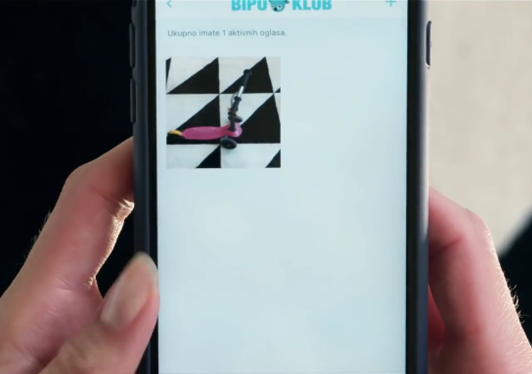
\includegraphics[height=0.15\textheight]{./slike/Picture3.png}
			\caption{ Pregled vlastitih oglasa u aplikaciji BIPO CLUB}
			\label{fig3}
		\end{figure}
		\newline
		Aplikacija korisniku omogućava pregled vlastitih oglasa - ova funkcionalnost bit će implementirana i u našoj web aplikaciji. Naime, ako korisnik ima predmet koji želi donirati, može to učiniti kreiranjem oglasa. Oglas se prije objave „šalje“ administratoru na pregled i ukoliko dobije zeleno svjetlo, oglas se objavljuje. Ako oglas nije valjan(nedostaju podaci ili su neispravni), administrator ga vraća korisniku na doradu, a ima i mogućnost odbiti oglas.\\
		\newline
		\begin{figure}[h!]
			\center
			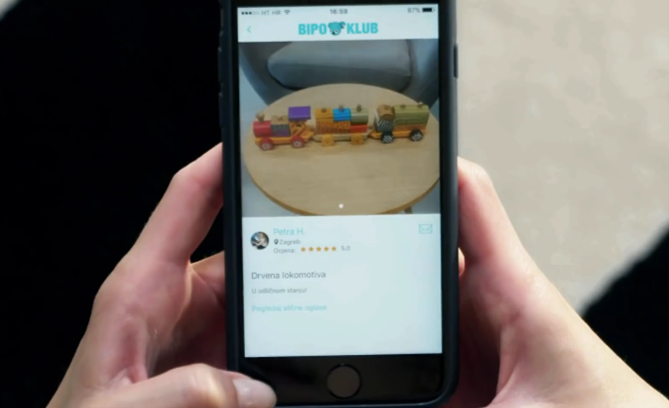
\includegraphics[height=0.15\textheight]{./slike/Picture4.png}
			\caption{ Pregled aktivnih oglasa u aplikaciji BIPO CLUB}
			\label{fig4}
		\end{figure}
		\newline
		Aplikacija omogućava pregled aktivnih oglasa- ova funkcionalnost bit će implementirana i u našoj web aplikaciji. \\
		\newline
		Na temelju podataka koje je korisnik unio o djeci, prikazuju mu se oglasi od najnovijih(do 3 dana starosti) prema najstarijima. Osim automatskog filtriranja koje rezultira preporučenim oglasima, korisnik će moći i ručno postaviti dodatne filtere za oglase (odabrati kategorije ili potkategorije). Uzmimo već navedeni primjer - osoba ima muško dijete u dobi od 3 godine i zanimaju je igračke za sina. U tom slučaju osoba će dodatno postaviti filter - odabrat će kategoriju dječjih igračaka, a iste će ponovo biti filtrirane prema dobi i spolu ako su oni definirani. \\
		\newline
		\begin{figure}[h!]
			\center
			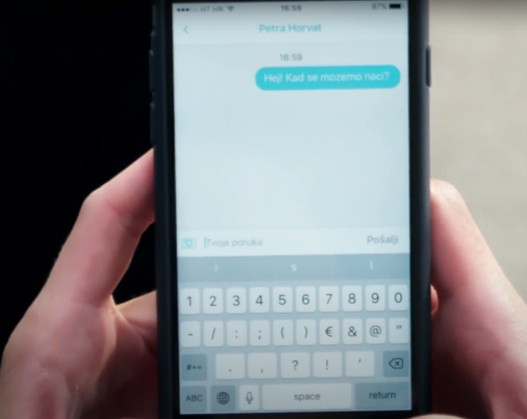
\includegraphics{./slike/Picture5.png}
			\caption{ Chat room s donatorom u aplikaciji BIPO CLUB}
			\label{fig5}
		\end{figure}
		\newline
		Aplikacija nudi direktno javljanje korisniku koji je postavio oglas kroz aplikaciju. Web aplikacija koja se razvija neće imati tu opciju te će se korisnici međusobno morati dogovarati van aplikacije.\\
		\newline
		Po primitku donacije počinje odbrojavanje do trenutka kada će aplikacija ponuditi primatelju da isti predmet proslijedi dalje. Odbrojavanje se temelji na istraženim podacima o vremenu korištenja određenih predmeta. Primjerice, znamo da se kolica 3u1 koriste 1,5 godina i po isteku tog vremena korisniku koji je primio kolica u obliku donacije iskočit će prozor s upitom želi li možda proslijediti kolica dalje (donirati kreiranjem oglasa) ako su ista još u dobrom stanju. \\
		\newline
		Osim BIPO CLUB mobilne aplikacije, postoje razne grupe na Facebook-u za razmjenu i prodaju dječjih stvari, kao i odjeljak na Njuškalu koji nudi razmjenu i prodaju dječjih predmeta.\\
		\newline
		\begin{figure}[h!]
			\center
			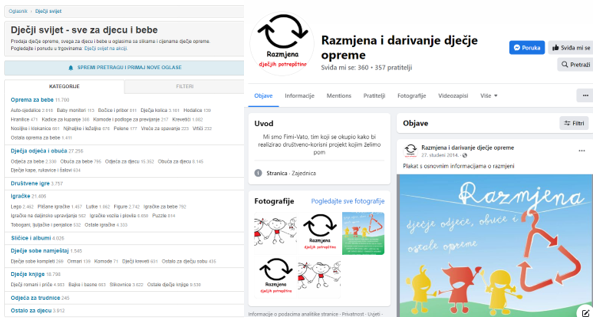
\includegraphics[width = \linewidth]{./slike/Picture6.png}
			\caption{Njuškalo (lijevo) i Facebook grupa (desno)}
			\label{fig6}
		\end{figure}
		\newline
		Na kraju ovog projekta cilj je imati funkcionalnu web aplikaciju za doniranje i primanje predmeta putem oglasa. Kao što smo do sada vidjeli, takve aplikacije trenutno ne postoje i naša su očekivanja da bi aplikacija brzo postala popularna. \\
		\newline
		Cijeli proces izrade počeo je analizom zahtjeva naručitelja, razradom funkcionalnih zahtjeva i izradom UML dijagrama (Use case dijagrama i sekvencijskih dijagrama), kao i ER modela baze podataka koja će čuvati sve podatke o korisnicima i pratiti oglase i razna dopuštenja. Rad se nastavlja programiranjem backenda i frontenda te obuhvaća pisanje popratne dokumentacije kao i testiranje same aplikacije u više faza i puštanje u pogon. Na kraju nas još očekuje prezentiranje same aplikacije i demonstracija implementiranih funkcionalnosti.\\
		\newline
		\eject
		Uvijek postoji mjesta za poboljšanje… Cijeli cilj ovog projekta je pomaganje zajednici tako da bi i nadogradnja aplikacije vodila k stvaranju sigurnije i ravnopravne zajednice korisnika. \\
		\newline
		Za veće zadovoljstvo korisnika, ali i kako bi maksimizirali uspješnost doniranja i spajanja donatora s korisnikom koji je prima, sljedeća nadogradnja aplikacije bila bi usmjerena prema sustavu ocjenjivanja donatora i primatelja donacija (dvosmjerno ocjenjivanje), kao i sustavu za prijavljivanje korisnika koji krše opća pravila aplikacije i/ili sabotiraju uspješno doniranje predmeta. Nažalost, uvijek ima ljudi koji žele iskoristiti druge ljude ili tuđu dobrotu. Kako bi smanjili mogućnost da jedan korisnik primi velik broj donacija u jako kratkom vremenu ili nelogičnu kombinaciju donacija (prema podacima o djeci) te potom dobivene predmete preproda, uložili bi u razvijanje sustava za praćenje primljenih donacija.\\
		\newline
		Cilj je imati što sigurniju zajednicu donatora i primatelja donacija, kao i ulagati u sustav za poticanje kruženja predmeta i stalan priljev korisnika. \\
		\newline
		Aplikacija bi omogućavala nadogradnje, kao i prilagodbu na mobilne uređaje i tablete.
		\eject
		